% Created 2023-08-14 lun 20:52
% Intended LaTeX compiler: pdflatex
\documentclass[11pt]{article}
\usepackage[utf8]{inputenc}
\usepackage[T1]{fontenc}
\usepackage{graphicx}
\usepackage{grffile}
\usepackage{longtable}
\usepackage{wrapfig}
\usepackage{rotating}
\usepackage[normalem]{ulem}
\usepackage{amsmath}
\usepackage{textcomp}
\usepackage{amssymb}
\usepackage{capt-of}
\usepackage{hyperref}
\usepackage{../modern}
\setcounter{secnumdepth}{2}
\author{Luis Eduardo Galindo Amaya}
\date{2023-08-14}
\title{Mapa conceptual tecnologías emergentes}
\hypersetup{
 pdfauthor={Luis Eduardo Galindo Amaya},
 pdftitle={Mapa conceptual tecnologías emergentes},
 pdfkeywords={},
 pdfsubject={},
 pdfcreator={Emacs 27.1 (Org mode 9.3)}, 
 pdflang={Spanish}}
\begin{document}


\newenvironment{onec}
               {
                 \begin{minipage}{0.18\textwidth}
                   \raggedright

                   \\
               }
               { 
                 \\\\
                 \end{minipage}
               }

\newenvironment{twoc}
               {
                 \begin{minipage}{0.39\textwidth}
                   \raggedright

                   \\
               }
               { 
                 \\\\
                 \end{minipage}
               }

\newenvironment{threec}
               {
                 \begin{minipage}{0.58\textwidth}
                   \raggedright

                   \\
               }
               { 
                 \\\\
                 \end{minipage}
               }

\begin{twoc}
\textbf{Tema}: \\
Mapa conceptual tecnologías emergentes
\end{twoc}
\begin{threec}
\textbf{Nombre}: Luis Eduardo Galindo Amaya \\
\textbf{Matricula}: 1274895 \\
\textbf{Fecha}: 2023-08-14 
\end{threec}


\noindent\rule{\textwidth}{0.5pt}
\vspace{\fill}
\begin{center}
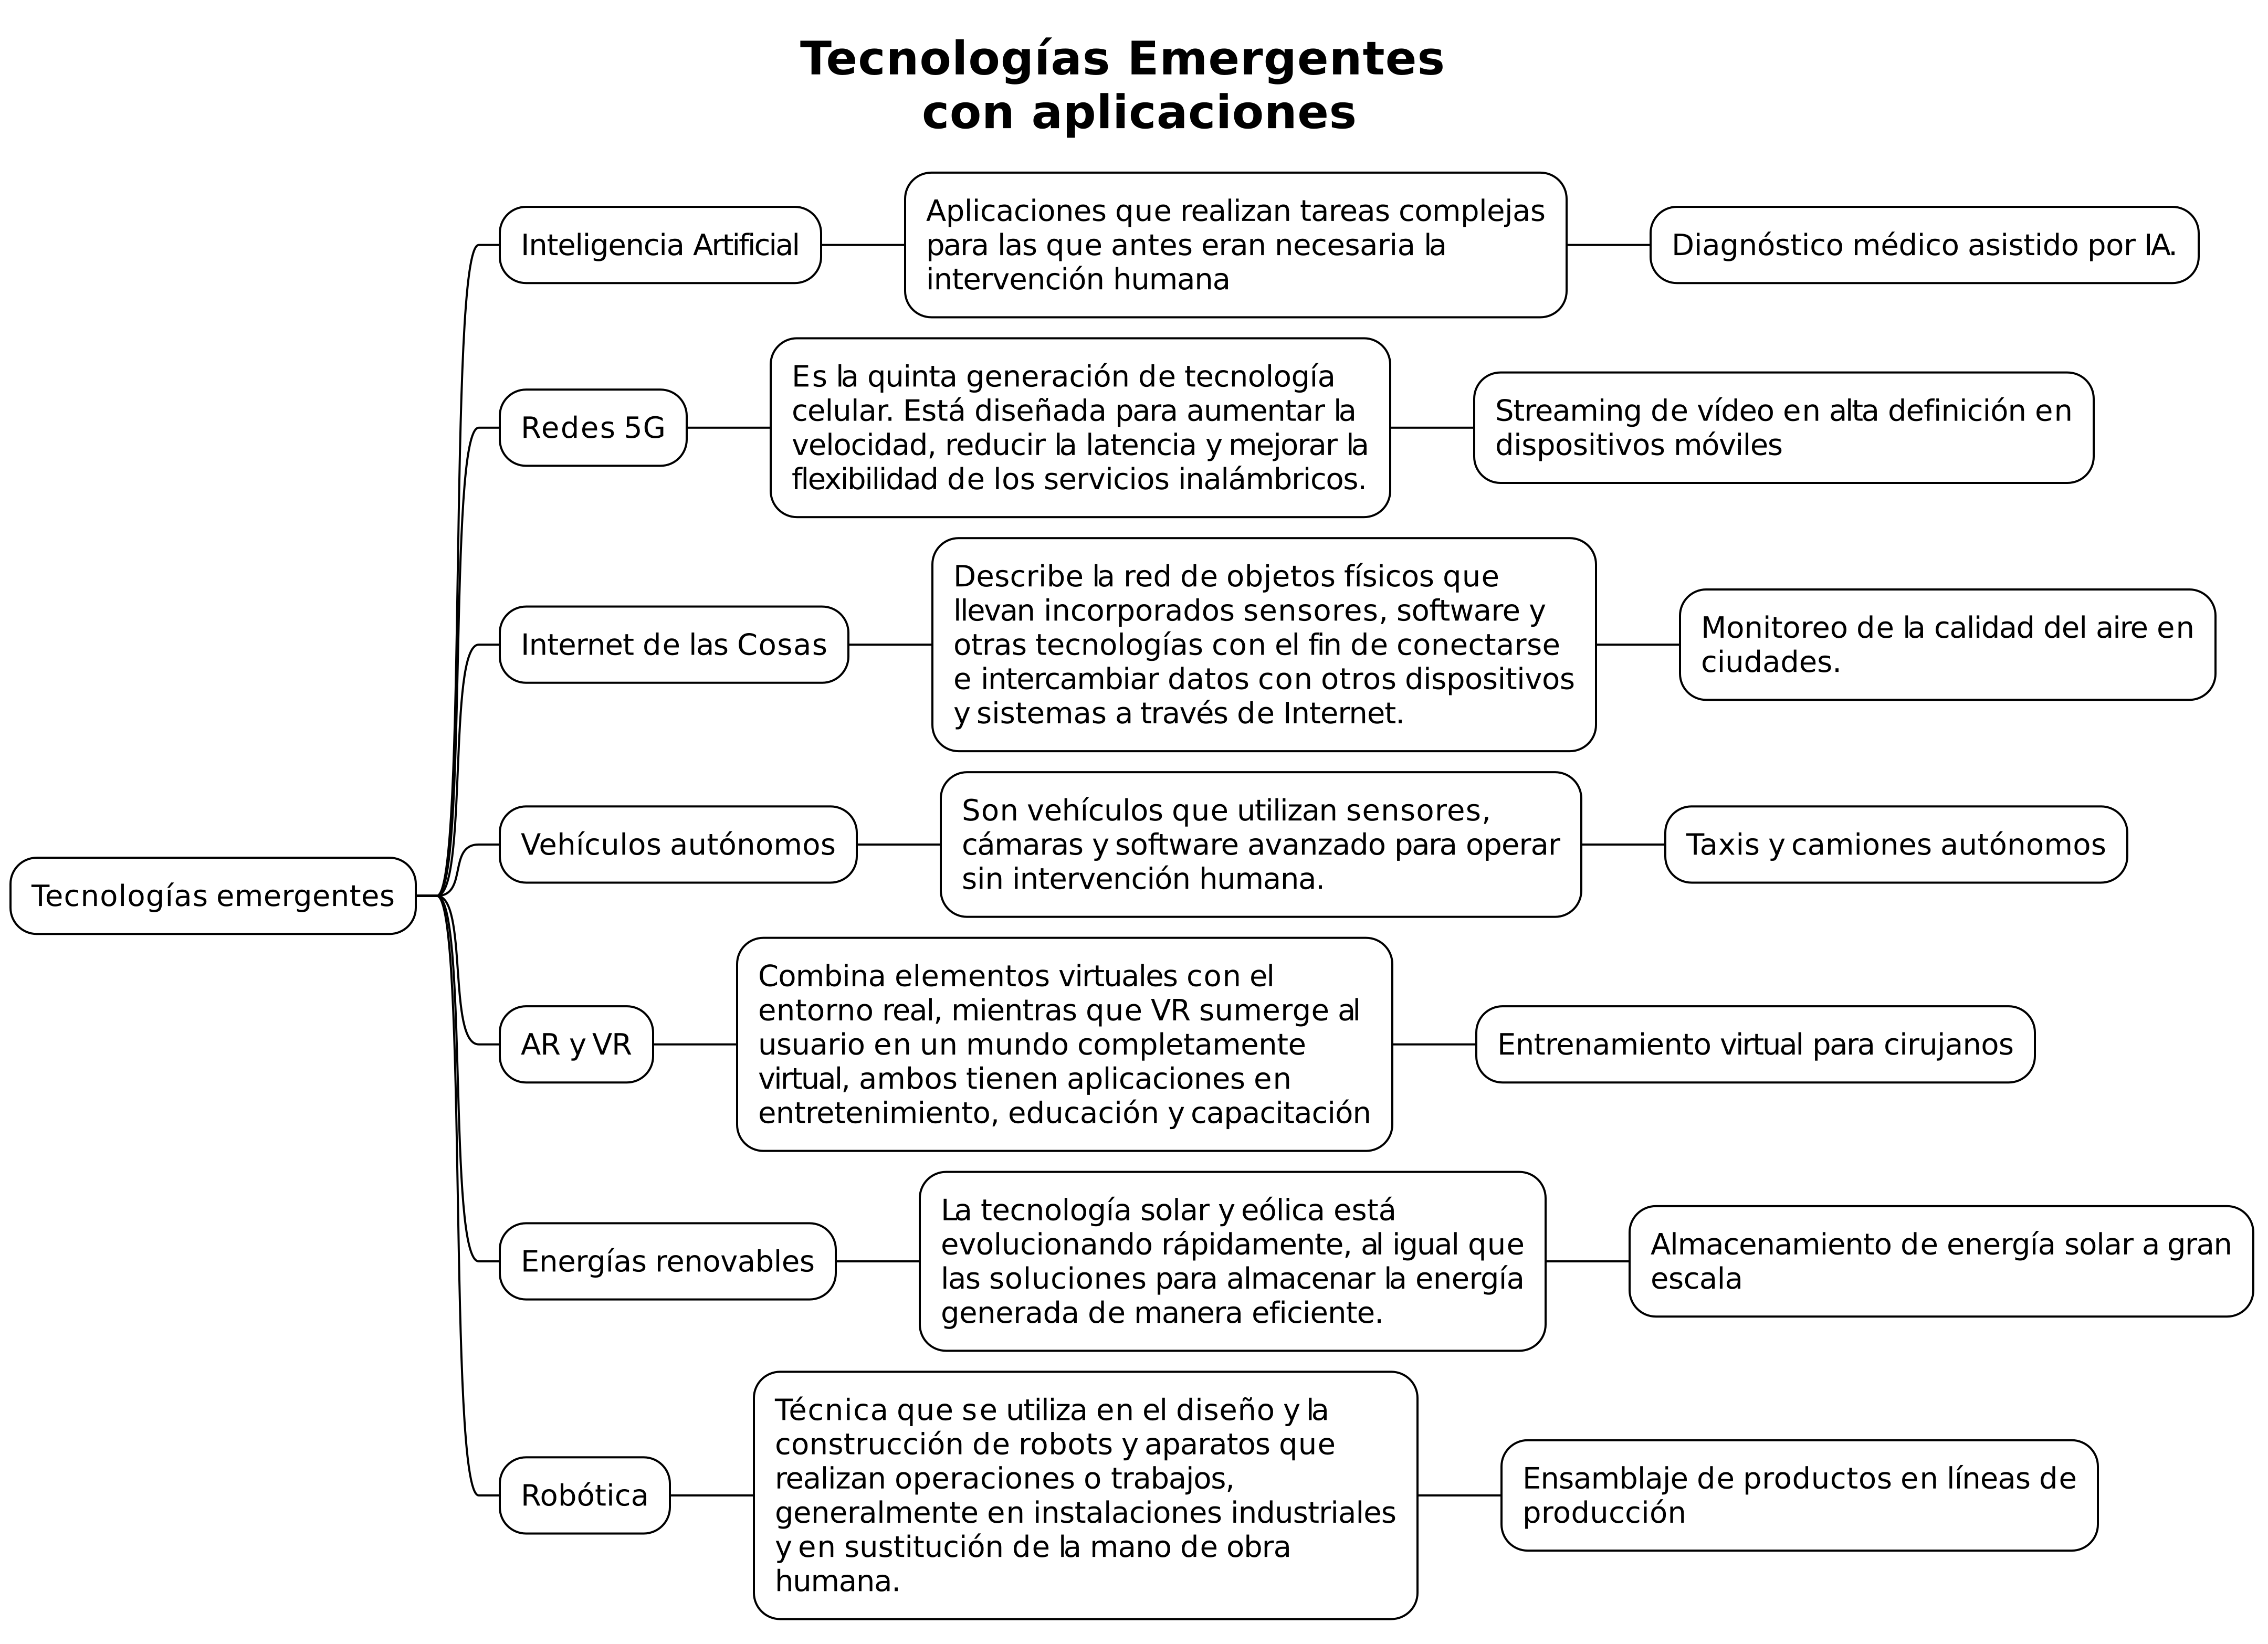
\includegraphics[width=.9\linewidth]{images/a.png}
\end{center}
\vspace{\fill}

Fuentes:
\begin{itemize}
\item \url{https://www.oracle.com/mx/artificial-intelligence/what-is-ai/}
\item \url{https://www.cisco.com/c/es\_mx/solutions/what-is-5g.html}
\item \url{https://www.oracle.com/mx/internet-of-things/what-is-iot/}
\item \url{https://www.kia.com/mx/discover-kika/ask/Are-self-driving-cars-the-future.html}
\item \url{https://es.wikipedia.org/wiki/Rob\%C3\%B3tica}
\end{itemize}
\end{document}
